\DontFrameThisInToc
\Annex{Annexe sur l'évaluation d'un \textit{clustering} à l'aide de la \texttt{v-measure}}
\label{annex:D-ANNEXE-EVALUATION-CLUSTERING}

	% INTRODUCTION DE L'ANNEXE.
	Au cours de nos études, nous avons besoin de comparer nos résultats de \textit{clustering} à une vérité terrain représentant la cible à atteindre au cours des itérations.
	Nous utilisons alors la \texttt{v-measure} (\cite{rosenberg-hirschberg:2007:vmeasure-conditional-entropybased}) pour discuter de la proximité du résultat d'une itération avec sa cible.
	
	% Annonce du plan et conseils.
	\begin{leftBarAuthorOpinion}
		Dans cette annexe, nous allons décrire la \texttt{v-measure} de manière formelle puis détailler son fonctionnement sur quelques exemples.
		Si la première section est très (\textit{voir trop}) abstraite, consultez directement la deuxième section : les exemples permettront d'illustrer les intuitions principales.
	\end{leftBarAuthorOpinion}
	
	% TABLE DES MATIÈRES DE L'ANNEXE.
	\minitoc

	%%%%%--------------------------------------------------------------------
	%%%%% Annexe D.1: Définition de la \texttt{v-measure}.
	%%%%%--------------------------------------------------------------------
	\newpage
	\section{Définition de la \texttt{v-measure}}
	\label{annex:D.1-ANNEXE-EVALUATION-CLUSTERING-DEFINITION}
		
		%%% NOTATIONS.
		Pour ces définitions, nous allons utiliser les notations suivantes :
		\begin{itemize}
			% Data.
			\item $\mathcal{D}$ représente l'ensemble des données $d$ à segmenter ;
			% Classes.
			\item $\mathcal{C}$ représente l'ensemble des classes $c$ de la vérité terrain (\textit{référence à atteindre}) ;
			% \textit{Cluster}.
			\item $\mathcal{K}$ représente l'ensemble des \textit{cluster} $k$ de la segmentation (\textit{clustering proposé par la machine à une itération donnée}).
		\end{itemize}
		
		
		%%% INTRODUCTION, ENTROPIE ET ENTROPIE CONDITIONNELLE.
		La \texttt{v-measure} entre un \textit{clustering} $\mathcal{K}$ et la vérité terrain $\mathcal{C}$ (servant de référence) est un score entropique calculé à partir de deux termes : l'homogénéité (\textit{homogeneity}) et la complétude (\textit{completeness}).
		Pour calculer ces termes, nous avons donc besoin d'introduire les concepts d'entropie intrinsèque et d'entropie conditionnelle.
		\newline
		
		% Description de l'entropie.
		L'\textbf{entropie intrinsèque} d'une segmentation $\mathcal{X}$ des données $\mathcal{D}$, notée $H(\mathcal{X})$, est définie comme l'opposé de la somme des termes $p(x) \cdot log~p(x)$,
		où $p(x)$ représente la proportion d'éléments de $\mathcal{D}$ contenu dans le groupe $x \in \mathcal{X}$.
		
		% Equation.
		\begin{equation}
			\label{equation:D.1-ANNEXE-EVALUATION-CLUSTERING-DEFINITION-ENTROPTY}
			H(\mathcal{X})~=~
				-
				\sum\limits_{
					x \in \mathcal{X}
				}
				\frac{
					|x|
				}{
					|\mathcal{D}|
				}
				\cdot
				\texttt{log} \Bigl(
					\frac{
						|x|
					}{
						|\mathcal{D}|
					}
				\Bigr)
		\end{equation}
		
		% Description de l'entropie conditionnelle.
		L'\textbf{entropie conditionnelle} d'une segmentation $\mathcal{X}$ par rapport à une autre segmentation $\mathcal{Y}$, notée $H(\mathcal{X}|\mathcal{Y})$, est un score compris entre $0$ et $H(\mathcal{X})$ qui est obtenu par l'opposé des sommes des termes $p(x \cap y) \cdot log~p(x \cap y|y)$,
		où $p(x \cap y)$ représente la proportion d'éléments de $\mathcal{D}$ contenus dans l'intersection $x \cap y$,
		et $p(x \cap y|y)$ représente la proportion d'éléments de $y$ contenus dans l'intersection $x \cap y$.
		
		% Equation.
		\begin{equation}
			\label{equation:D.1-ANNEXE-EVALUATION-CLUSTERING-DEFINITION-ENTROPTY-CONDITIONNELLE}
			H(\mathcal{X}|\mathcal{Y})~=~
				-
				\sum\limits_{
					x \in \mathcal{X}
				}
				\sum\limits_{
					y \in \mathcal{Y}
				}
				\frac{
					|x \cap y|
				}{
					|\mathcal{D}|
				}
				\cdot
				\texttt{log} \Bigl(
					\frac{
						|x \cap y|
					}{
						|y|
					}
				\Bigr)
		\end{equation}
		
		% Interprétation.
		\begin{leftBarAuthorOpinion}
			La notion d'entropie est difficile à appréhender, mais nous proposons toutefois les pistes d'interprétation suivantes :
			\begin{itemize}
				\item l'entropie intrinsèque $H(\mathcal{X})$ représente le "\textbf{désordre}" de la segmentation $\mathcal{X}$ :
				en effet, si les données seront réparties dans un grand nombre de groupes ou dans des groupes déséquilibrés, alors il y aura plus de termes $p(x) \cdot log p(x)$, et donc l'entropie sera plus grande ;
				\item l'entropie conditionnelle $H(\mathcal{X}|\mathcal{Y})$ représente à quel point une segmentation $\mathcal{X}$ \textbf{ne respecte pas une autre segmentation} $\mathcal{Y}$ :
				en effet, si $\mathcal{X}$ respecte $\mathcal{Y}$, alors les intersections non nulles entre $\mathcal{X}$ et $\mathcal{Y}$ ressembleront davantage aux groupes de $\mathcal{Y}$ et les termes $log~p(x \cap y|y)$ seront davantage nuls, donc l'entropie conditionnelle sera plus faible.
			\end{itemize}
		\end{leftBarAuthorOpinion}
		
		%%% HOMOGENEITE et COMPLETUDE
		\newpage
		% Description de l'homogénéité.
		L'\textbf{homogénéité} d'un \textit{clustering} $\mathcal{K}$ par rapport à la vérité terrain $\mathcal{C}$ (servant de référence), notée $\texttt{homogeneity}(C|K)$, est un score entre $0$ et $1$ qui est obtenu par $1$ moins le ratio entre :
		\begin{itemize}
			\item l'entropie conditionnelle de la vérité terrain $\mathcal{C}$ par rapport au \textit{clustering} $\mathcal{K}$, et
			\item l'entropie intrinsèque de la vérité terrain $\mathcal{C}$.
		\end{itemize}
		
		% Equation.
		\begin{equation}
			\label{equation:D.1-ANNEXE-EVALUATION-CLUSTERING-DEFINITION-HOMEGENEITE}
			\texttt{homogeneity}(\mathcal{C}|\mathcal{K})~=~
				1
				-
				\frac{
					H(\mathcal{C}|\mathcal{K})
				}{
					H(\mathcal{C})
				}
		\end{equation}
		
		% Description de la complétude.
		La \textbf{complétude} d'un \textit{clustering} $\mathcal{K}$ par rapport à la vérité terrain $\mathcal{C}$ (servant de référence), notée $\texttt{completeness}(C|K)$, est un score entre $0$ et $1$ qui est obtenu par $1$ moins le ratio entre :
		\begin{itemize}
			\item l'entropie conditionnelle du \textit{clustering} $\mathcal{K}$ par rapport à la vérité terrain $\mathcal{C}$, et
			\item l'entropie intrinsèque du \textit{clustering} $\mathcal{K}$.
		\end{itemize}
		
		% Equation.
		\begin{equation}
			\label{equation:D.1-ANNEXE-EVALUATION-CLUSTERING-DEFINITION-COMPLETENESS}
			\texttt{completeness}(\mathcal{C}|\mathcal{K})~=~
				1
				-
				\frac{
					H(\mathcal{K}|\mathcal{C})
				}{
					H(\mathcal{K})
				}
		\end{equation}
		
		% Interprétation.
		\begin{leftBarAuthorOpinion}
			Nous pouvons interpréter ces termes de la manière suivante :
			\begin{itemize}
				\item l'homogénéité $\texttt{homogeneity}(\mathcal{C}|\mathcal{K})$ représente à quel point \textbf{chaque \textit{cluster} $k$ contient uniquement des données provenant d'une même et une seule classe $c$} :
				en effet, l'homogénéité est maximale lorsque l'entropie conditionnelle $H(\mathcal{C}|\mathcal{K})$ minimale, et cette entropie conditionnelle est nulle si chaque \textit{cluster} $k$ ne contient que des données d'une même classe $c$ ($log \frac{|k|}{|k|}=log(1)=0$) ;
				\item la complétude $\texttt{completeness}(\mathcal{C}|\mathcal{K})$ représente à quel point \textbf{chaque classe $c$ est contenue entièrement dans un même et unique \textit{cluster} $k$} :
				en effet, la complétude est maximale lorsque l'entropie conditionnelle $H(\mathcal{K}|\mathcal{C})$ minimale, et cette entropie conditionnelle est nulle si chaque classe $c$ ne contient que des données d'un même \textit{cluster} $k$ ;
				\item ces termes sont liés : $\texttt{homogeneity}(\mathcal{C}|\mathcal{K}) = \texttt{completeness}(\mathcal{K}|\mathcal{C})$ ($log \frac{|c|}{|c|}=log(1)=0$).
			\end{itemize}
		\end{leftBarAuthorOpinion}
		
		%%% VMEASURE
		
		% Description du calcul.
		La \textbf{V-Measure} d'un \textit{clustering} $\mathcal{K}$ par rapport à la vérité terrain $\mathcal{C}$ (servant de référence), notée $\texttt{v-measure}(C|K)$, est un score entre $0$ et $1$ qui est obtenu par la moyenne harmonique entre l'homogénéité et la complétude.
		
		% Equation.
		\begin{equation}
			\label{equation:D.1-ANNEXE-EVALUATION-CLUSTERING-DEFINITION-VMEASURE}
			\texttt{v-measure}(C|K)~=~2 \cdot \frac{
				\texttt{homogeneity}(\mathcal{C}|\mathcal{K}) \cdot \texttt{completeness}(\mathcal{C}|\mathcal{K})
			}{
				\texttt{homogeneity}(\mathcal{C}|\mathcal{K}) + \texttt{completeness}(\mathcal{C}|\mathcal{K})
			}
		\end{equation}
		
		% Interprétation.
		\begin{leftBarAuthorOpinion}
			Ce score de \texttt{v-measure} est le compromis entre l'homogénéité et la complétude.
			Pour être maximal, il faut que chaque \textit{cluster} ne contienne que des données d'une même classe et qu'en échange chaque classe ne soit contenue que dans un seul \textit{cluster}.
			Autrement dit : la \texttt{v-measure} est maximale si et seulement si chaque \textit{cluster} a une classe équivalente et inversement.
			
			Ce score est symétrique : $\texttt{v-measure}(C|K) = \texttt{v-measure}(K|C)$.
		\end{leftBarAuthorOpinion}

	%%%%%--------------------------------------------------------------------
	%%%%% Annexe D.2: Quelques exemples de calcul avec la \texttt{v-measure}.
	%%%%%--------------------------------------------------------------------
	\newpage
	\section{Quelques exemples de calcul avec la \texttt{v-measure}}
	\label{annex:D.2-ANNEXE-EVALUATION-CLUSTERING-EXEMPLE-VMEASURE}
		
		% Exemple 0 : Introduction
		Prenons quelques exemples pour illustrer les calculs d'homogénéité, de complétude et de \texttt{v-measure}.
		Pour cela, nous considérons le jeu d'exemples de $10$ objets, représentés en \textsc{Figure~\ref{figure:D.2-ANNEXE-EVALUATION-CLUSTERING-EXEMPLE-VMEASURE-0-PRESENTATION}} \textbf{(1)}, que nous voulons regrouper par forme (\texttt{carrés}, \texttt{ronds}, \texttt{triangles}), comme dans la \textsc{Figure~\ref{figure:D.2-ANNEXE-EVALUATION-CLUSTERING-EXEMPLE-VMEASURE-0-PRESENTATION}} \textbf{(2)}.
		%
		\begin{figure}[H]
			\centering
			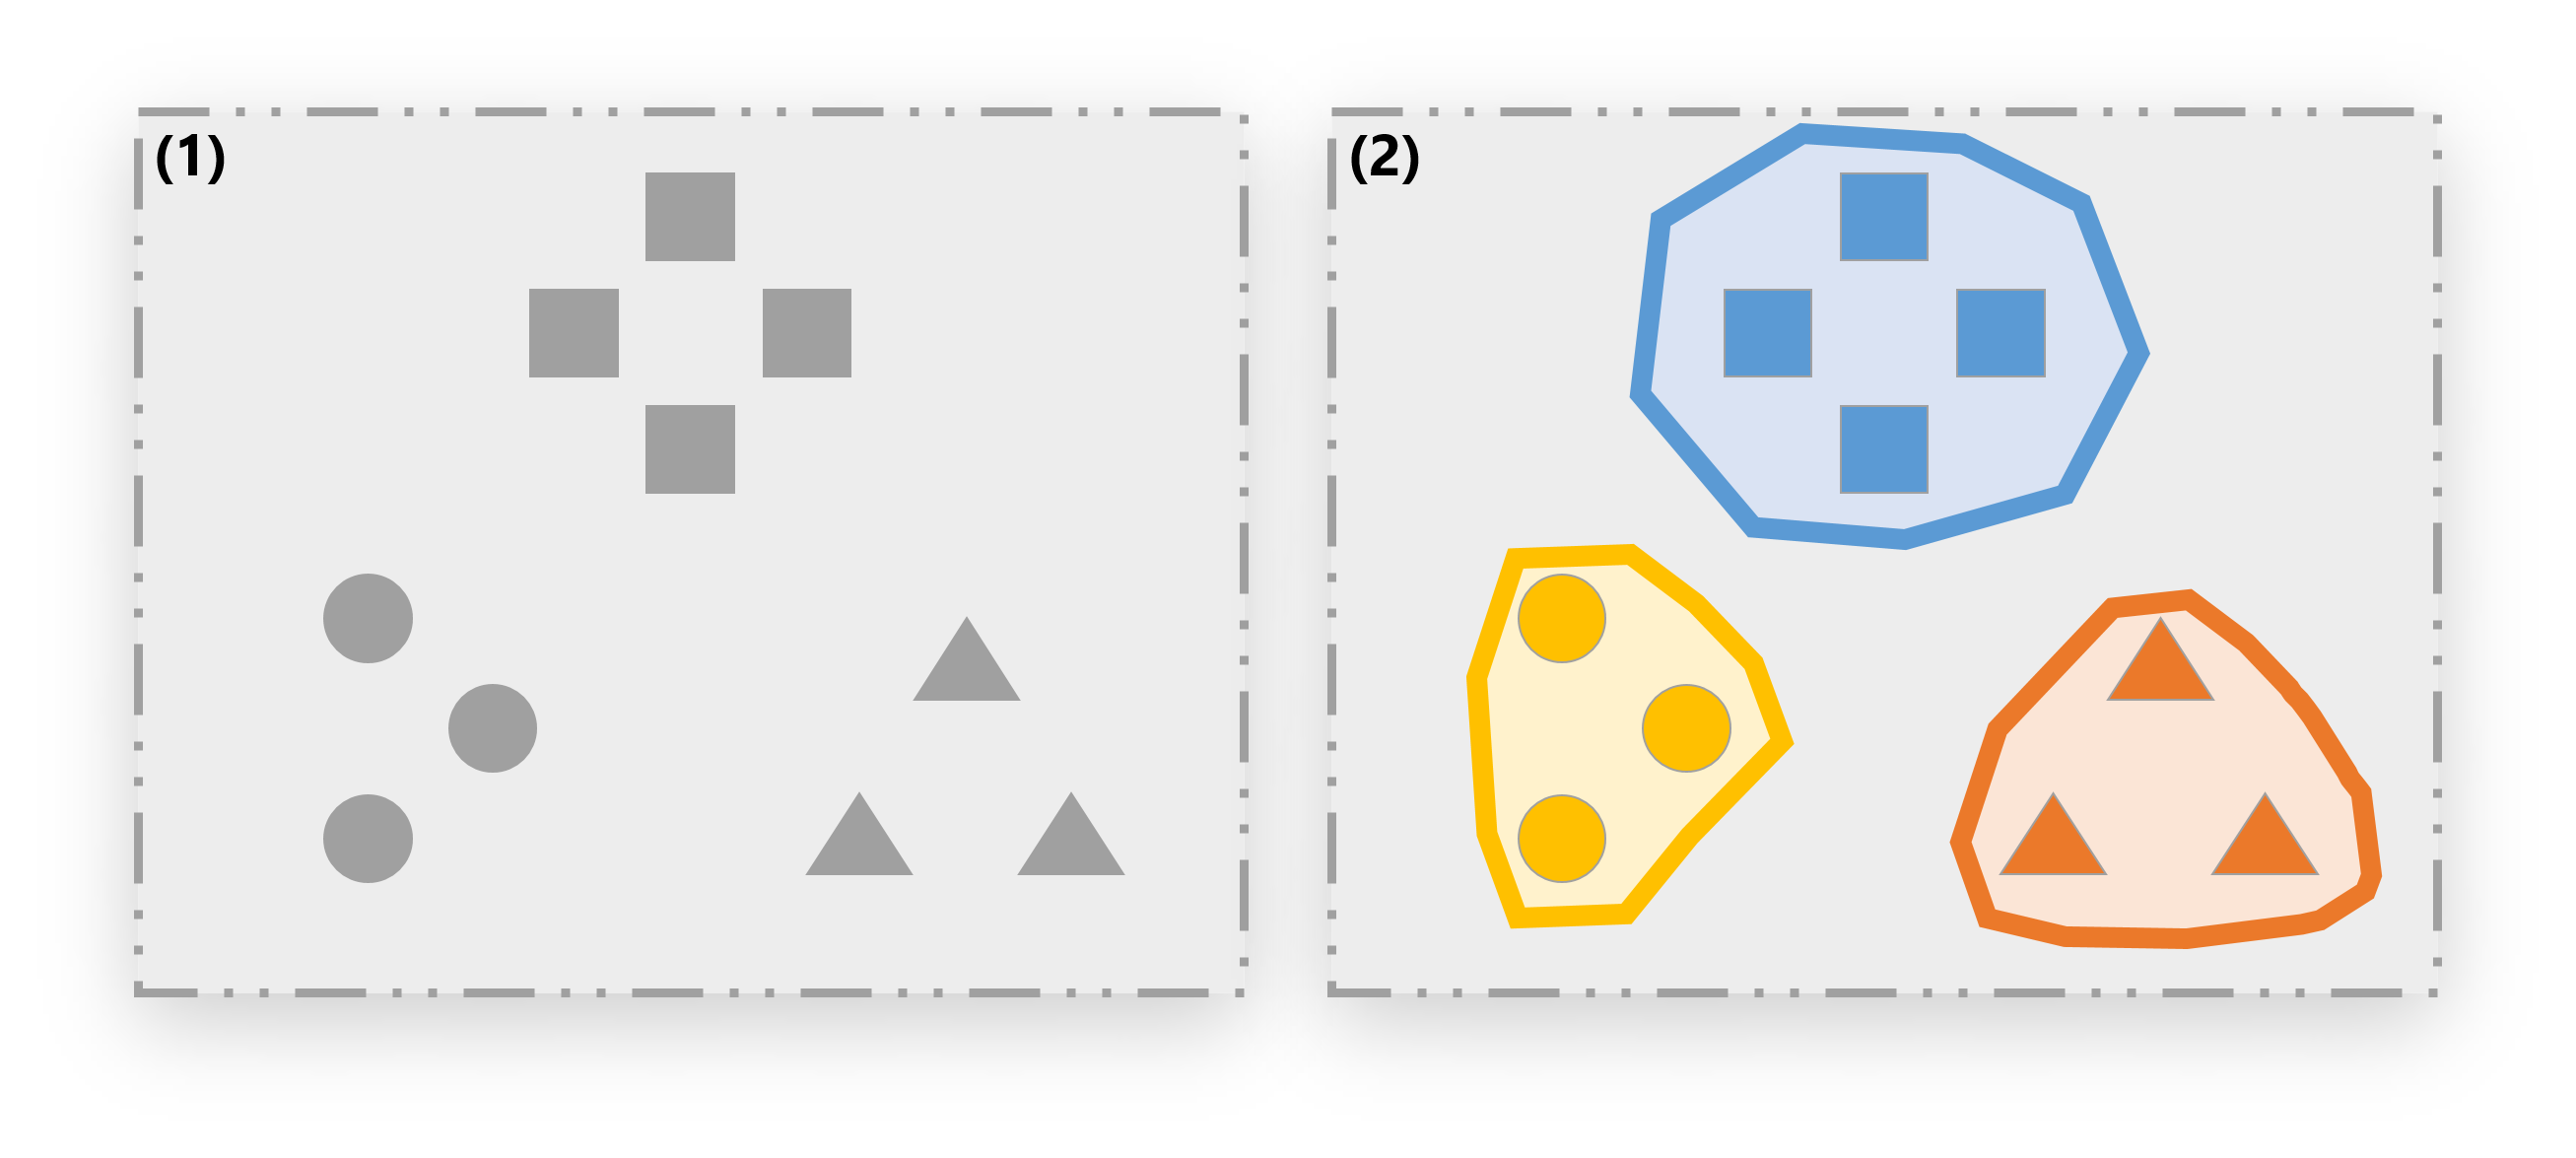
\includegraphics[width=0.95\textwidth]{figures/annexe-vmeasure-presentation}
			\caption{
				Présentation du jeu d'exemple :
				\textbf{(1)} représente $10$ données non regroupées ;
				\textbf{(2)} représente ces $10$ données regroupées en $3$ \textit{cluster} en fonction de formes : \texttt{carrés}, \texttt{ronds}e t \texttt{triangles}.
			}
			\label{figure:D.2-ANNEXE-EVALUATION-CLUSTERING-EXEMPLE-VMEASURE-0-PRESENTATION}
		\end{figure}
		
		% Segmentation parfaite.
		La \textbf{segmentation parfaite} de ces objets suivant leur forme est visible en \textsc{Figure~\ref{figure:D.2-ANNEXE-EVALUATION-CLUSTERING-EXEMPLE-VMEASURE-0-PRESENTATION}} \textbf{(2)}.
		En effet, nous pouvons voir que :
		\begin{itemize}
			\item ce \textit{clustering} est \textbf{homogène} ($homogeneity=1.00$) : il n'y a que des \texttt{carrés} dans le \textit{cluster} \textbf{\textcolor{colorSilverLakeBlue}{bleu}}, il n'y a que des \texttt{ronds} dans le \textit{cluster} \textbf{\textcolor{colorMinionYellow}{jaune}} et il n'y a que des \texttt{triangles} dans le \textit{cluster} \textbf{\textcolor{colorCarrotOrange}{orange}} ;
			\item ce \textit{clustering} est \textbf{complet} ($completeness=1.00$) : tous les \texttt{carrés} sont dans le \textit{cluster} \textbf{\textcolor{colorSilverLakeBlue}{bleu}}, tous les \texttt{ronds} sont dans le \textit{cluster} \textbf{\textcolor{colorMinionYellow}{jaune}} et tous les \texttt{triangles} sont dans le \textit{cluster} \textbf{\textcolor{colorCarrotOrange}{orange}} ;
			\item le \textit{clustering} \textbf{\textcolor{colorSilverLakeBlue}{bleu}}/\textbf{\textcolor{colorMinionYellow}{jaune}}/\textbf{\textcolor{colorCarrotOrange}{orange}} correspond donc parfaitement à sa vérité terrain \texttt{carrés}/\texttt{ronds}/\texttt{triangles} ($\texttt{v-measure}=1.00$).
		\end{itemize}
	
		% Exemple 1: Cas extrêmes
		\newpage
		\begin{figure}[H]
			\centering
			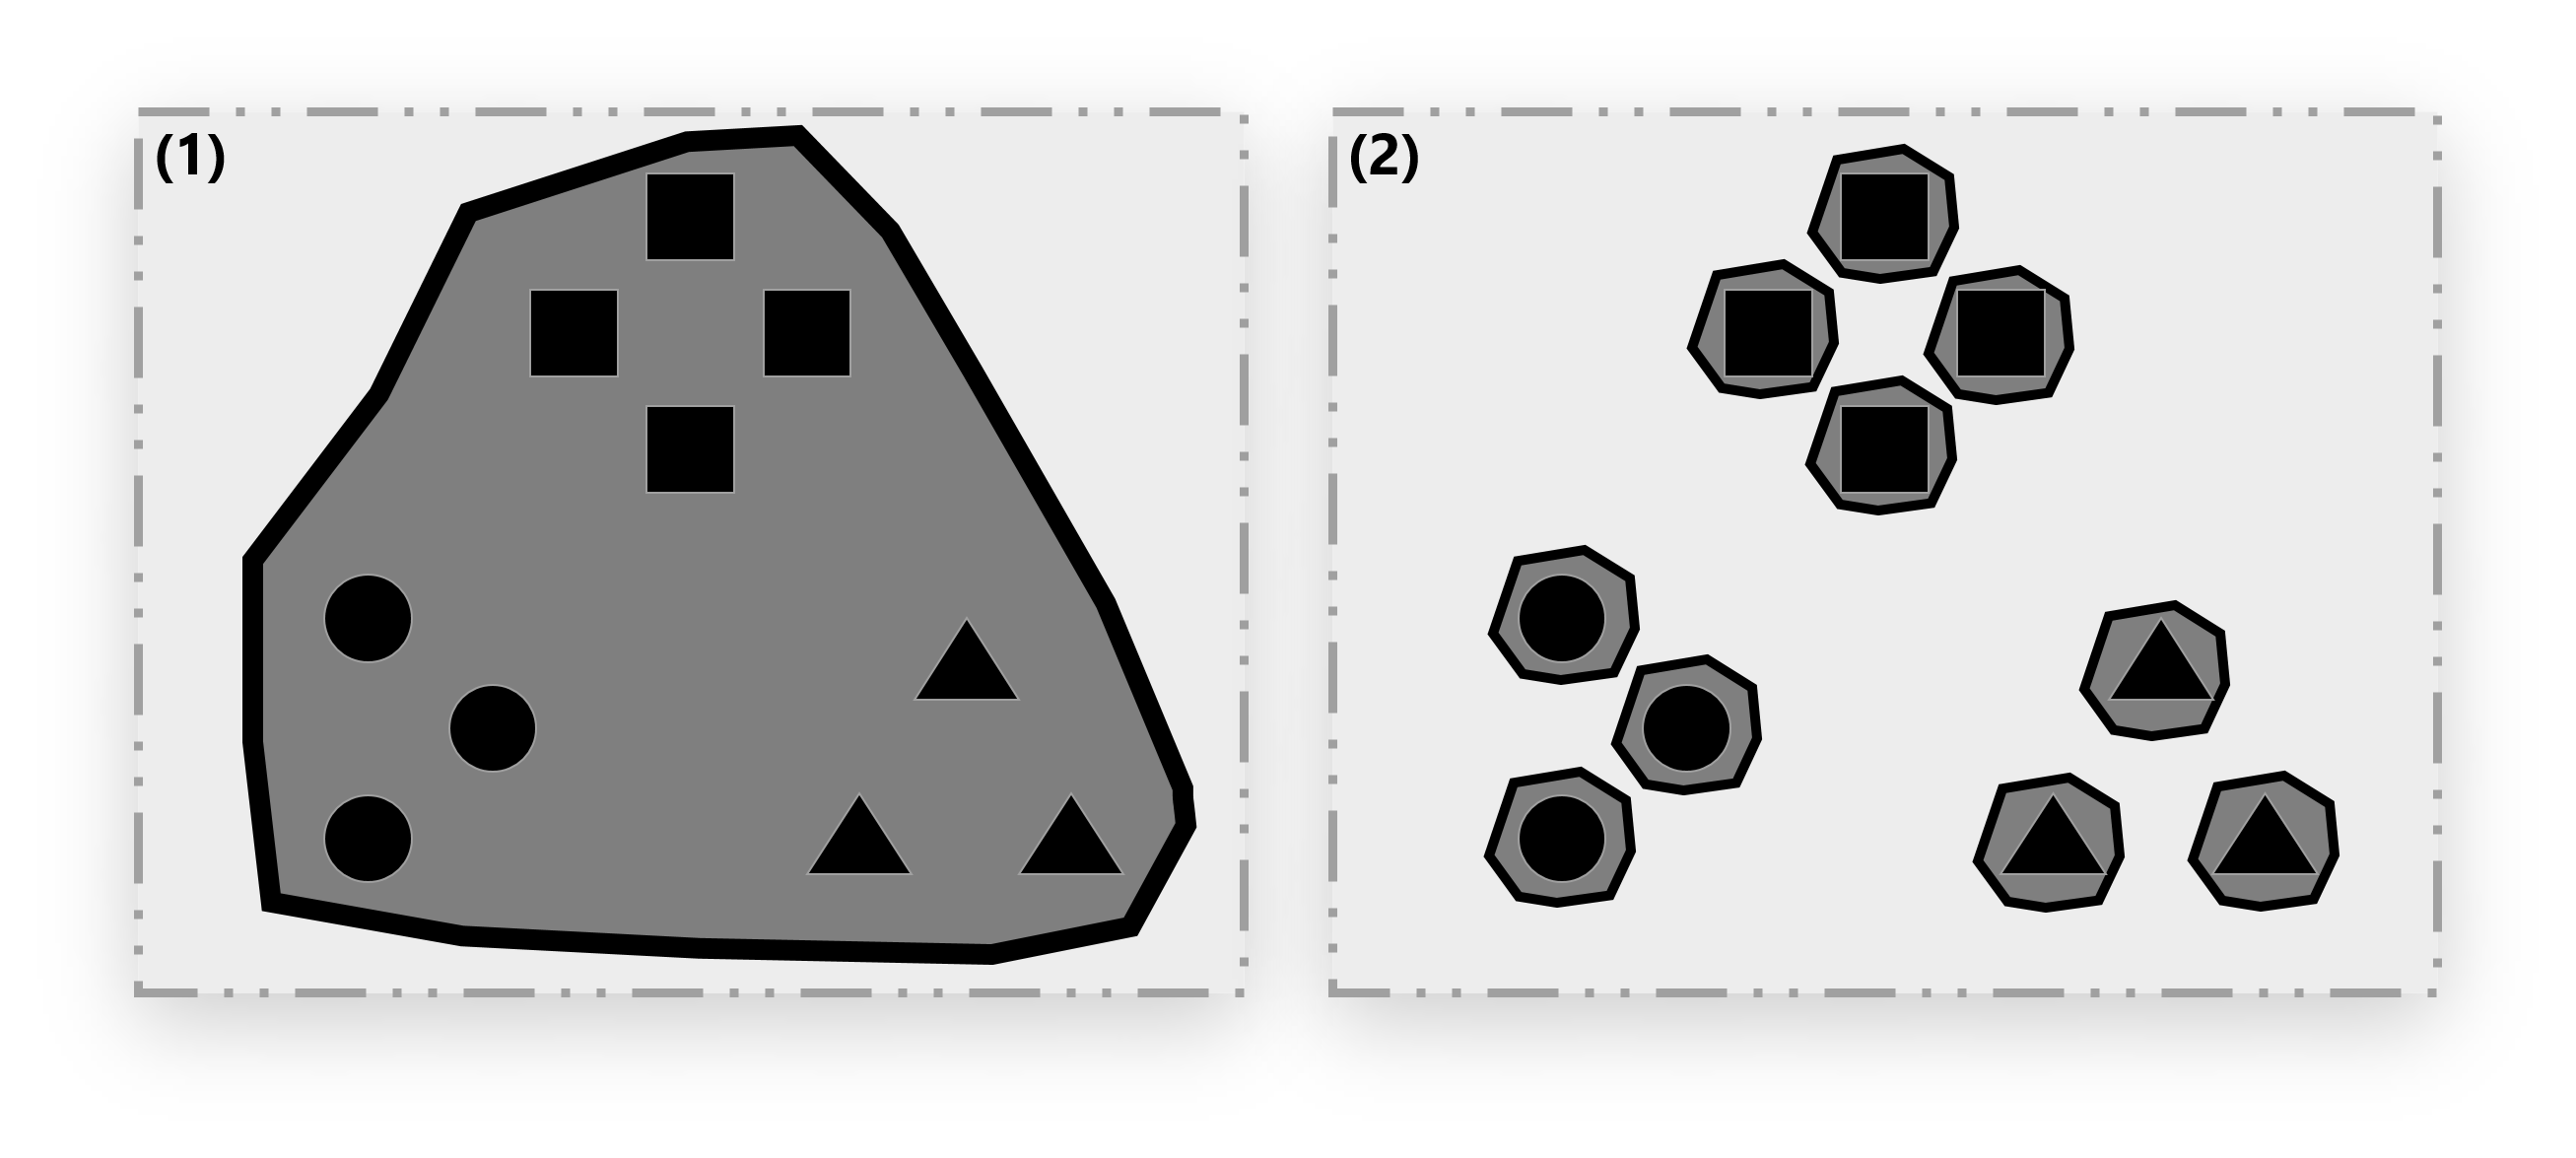
\includegraphics[width=0.95\textwidth]{figures/annexe-vmeasure-cas-extremes}
			\caption{
				Exemples de \texttt{clustering} avec des cas extrêmes :
				\textbf{(1)} représente un regroupement en un unique \textit{cluster} contenant toutes les données ;
				\textbf{(2)} représente un regroupement en $10$ \textit{cluster} où chaque \textit{cluster} contient une seule donnée.
			}
			\label{figure:D.2-ANNEXE-EVALUATION-CLUSTERING-EXEMPLE-VMEASURE-1-CAS-EXTREME}
		\end{figure}
		
		% Description des cas extrêmes.
		Prenons maintenant les deux cas extrêmes de la \textsc{Figure~\ref{figure:D.2-ANNEXE-EVALUATION-CLUSTERING-EXEMPLE-VMEASURE-1-CAS-EXTREME}}.
		\begin{itemize}
			\item \textbf{(1)} représente une segmentation où toutes les données sont regroupées dans un seul \textit{cluster} :
			\begin{itemize}
				\item ce \textit{clustering} est \textbf{complet} ($completeness=1.00$) : tous les \texttt{carrés} sont dans cet unique \textit{cluster}, tous les \texttt{ronds} sont dans cet unique \textit{cluster} et tous les \texttt{triangles} sont dans cet unique \textit{cluster} ;
				\item ce \textit{clustering} n'est \textbf{pas homogène} ($homogeneity=0.00$) : cet unique \textit{cluster} contient à la fois des \texttt{carrés}, des \texttt{ronds} et des \texttt{triangles} ;
				\item la \texttt{v-measure} finale est de $0.00$, confirmant que ce \textit{clustering} simpliste n'est pas performant car il n'est pas homogène.
			\end{itemize}
			\item \textbf{(2)} représente une segmentation où chaque donnée a son propre \textit{cluster} :
			\begin{itemize}
				\item ce \textit{clustering} est \textbf{homogène} ($homogeneity=1.00$) : comme chaque \textit{cluster} ne contient qu'une seule donnée, donc chaque \textit{cluster} ne contient que des données de la même forme ;
				\item ce \textit{clustering} n'est pas \textbf{complet} ($completeness=0.00$) : tous les \texttt{carrés} ne sont pas dans un même \textit{cluster}, tous les \texttt{ronds} ne sont pas dans un même \textit{cluster} et tous les \texttt{triangles} ne sont pas dans un même \textit{cluster} ;
				\item la \texttt{v-measure} finale est de $0.00$, confirmant que ce \textit{clustering} simpliste n'est pas performant car il n'est pas complet.
			\end{itemize}
		\end{itemize}
	
		% Exemple 2: Cas simples.
		\newpage
		\begin{figure}[H]
			\centering
			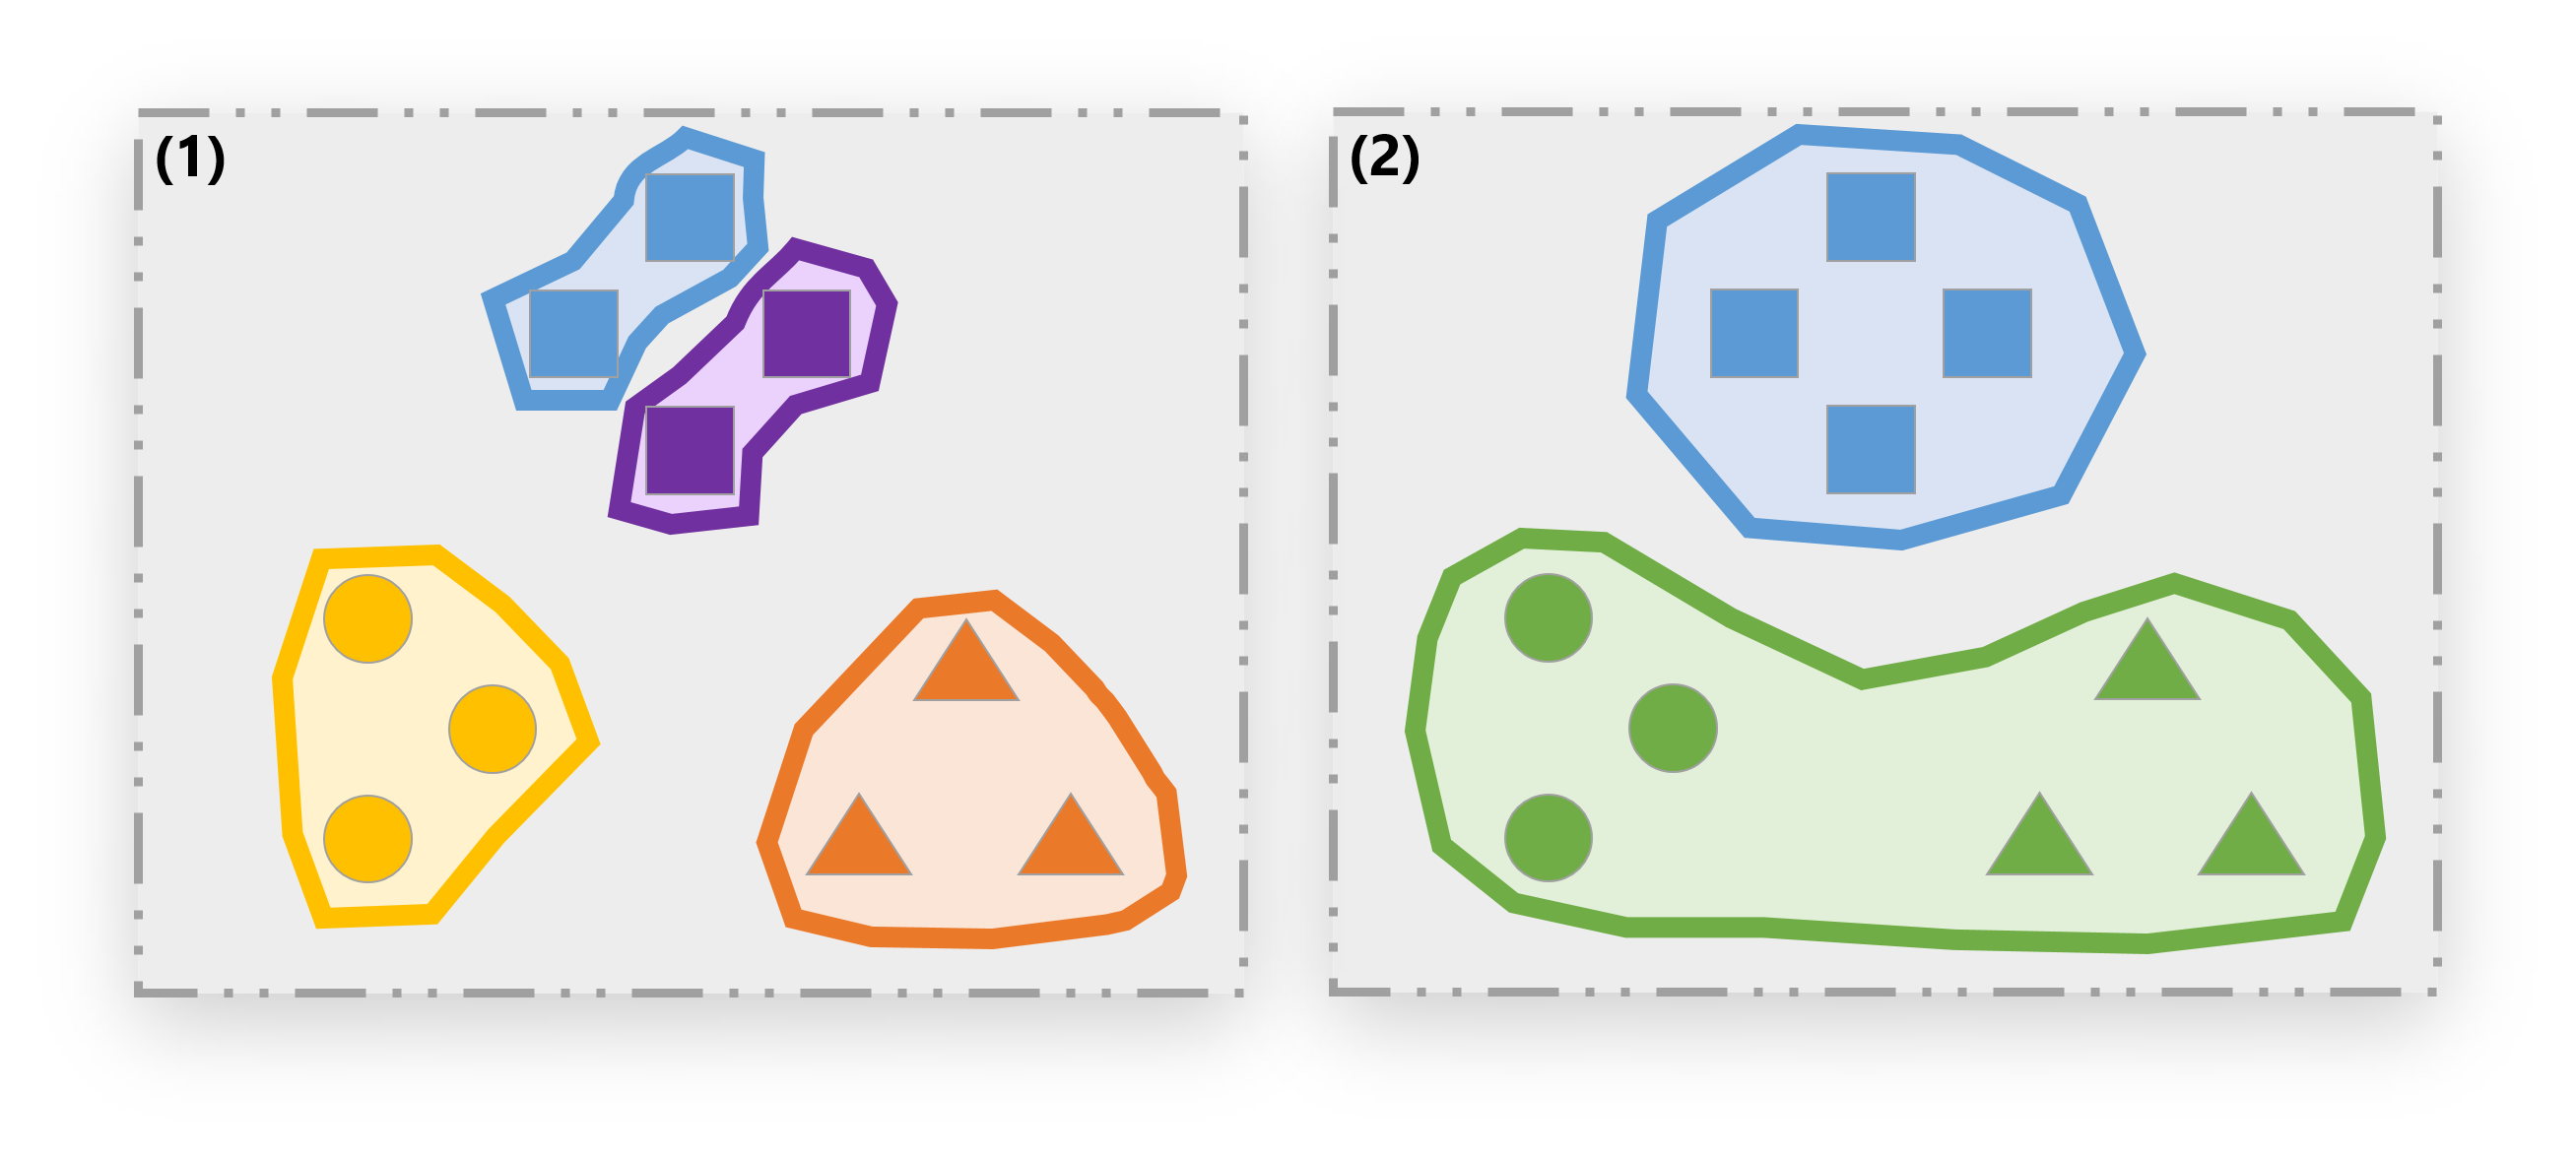
\includegraphics[width=0.95\textwidth]{figures/annexe-vmeasure-cas-simples}
			\caption{
				Exemples de \texttt{clustering} avec des cas simples :
				\textbf{(1)} représente un regroupement en $4$ \textit{cluster} où les \texttt{ronds} et les \texttt{triangles} sont correctement regroupés, mais où les \texttt{carrés} sont séparés.
				\textbf{(2)} représente un regroupement en $2$ \textit{cluster} où les \texttt{carrés} sont correctement regroupés, mais où les \texttt{ronds} et les \texttt{triangles} ont été rassemblés.
			}
			\label{figure:D.2-ANNEXE-EVALUATION-CLUSTERING-EXEMPLE-VMEASURE-2-CAS-SIMPLES}
		\end{figure}
		
		% Description des cas simples.
		Terminons maintenant les deux cas simples de la \textsc{Figure~\ref{figure:D.2-ANNEXE-EVALUATION-CLUSTERING-EXEMPLE-VMEASURE-2-CAS-SIMPLES}}.
		\begin{itemize}
			\item \textbf{(1)} représente une segmentation presque parfaite où les \texttt{carrés} sont séparés :
			\begin{itemize}
				\item ce \textit{clustering} est \textbf{homogène} ($homogeneity=1.00$) : il n'y a que des \texttt{carrés} dans le \textit{cluster} \textbf{\textcolor{colorSilverLakeBlue}{bleu}}, il n'y a que des \texttt{carrés} dans le \textit{cluster} \textbf{\textcolor{colorDarkPastelPurple}{violet}}, il n'y a que des \texttt{carrés} dans le \textit{cluster} \textbf{\textcolor{colorMinionYellow}{jaune}} et il n'y a que des \texttt{carrés} dans le \textit{cluster} \textbf{\textcolor{colorCarrotOrange}{orange}} ;
				\item ce \textit{clustering} n'est \textbf{pas assez complet} ($completeness=0.78$) : tous les \texttt{ronds} sont dans le \textit{cluster} \textbf{\textcolor{colorMinionYellow}{jaune}} et tous les \texttt{triangles} sont dans le \textit{cluster} \textbf{\textcolor{colorCarrotOrange}{orange}}, mais les \texttt{carrés} sont séparés dans les \textit{cluster} \textbf{\textcolor{colorSilverLakeBlue}{bleu}} et \textbf{\textcolor{colorDarkPastelPurple}{violet}} ;
				\item le score de \texttt{v-measure} final n'est de $0.89$, pénalisé par le manque de complétude des \textit{cluster} \textbf{\textcolor{colorSilverLakeBlue}{bleu}} et \textbf{\textcolor{colorDarkPastelPurple}{violet}}.
			\end{itemize}
			\item \textbf{(2)} représente une segmentation presque parfaite où les \texttt{ronds} et les \texttt{triangles} ont été rassemblés :
			\begin{itemize}
				\item ce \textit{clustering} est \textbf{complet} ($completeness=1.00$) : tous les \texttt{carrés} sont dans le \textit{cluster} \textbf{\textcolor{colorSilverLakeBlue}{bleu}}, tous les \texttt{ronds} sont dans le \textit{cluster} \textbf{\textcolor{colorDarkPastelGreen}{vert}} et tous les \texttt{triangles} sont dans le \textit{cluster} \textbf{\textcolor{colorDarkPastelGreen}{vert}} ;
				\item ce \textit{clustering} n'est \textbf{pas assez homogène} ($completeness=0.62$) : il n'y a que des \texttt{carrés} dans le \textit{cluster} \textbf{\textcolor{colorSilverLakeBlue}{bleu}}, mais il y a à la fois des \texttt{ronds} et des \texttt{triangles} dans le \textit{cluster} \textbf{\textcolor{colorDarkPastelGreen}{vert}} ;
				\item le score de \texttt{v-measure} final n'est de $0.76$, pénalisé par le manque d'homogénéité du \textit{cluster} \textbf{\textcolor{colorDarkPastelGreen}{vert}}.
			\end{itemize}
		\end{itemize}
	
	